\documentclass[12pt,twoside]{article}
\usepackage{amsmath, amssymb}
\usepackage{amsmath}
\usepackage[active]{srcltx}
\usepackage{amssymb}
\usepackage{amscd}
\usepackage{makeidx}
\usepackage{float}
\usepackage{amsthm}
\usepackage{algpseudocode}
\usepackage{algorithm}
\usepackage{graphicx}
\usepackage[spanish, es-tabla]{babel}
\usepackage{multirow}
\usepackage{cite}
\renewcommand{\baselinestretch}{1}
\graphicspath{{images/}}
\setcounter{page}{1}
\setlength{\textheight}{21.6cm}
\setlength{\textwidth}{14cm}
\setlength{\oddsidemargin}{1cm}
\setlength{\evensidemargin}{1cm}
\pagestyle{myheadings}
\thispagestyle{empty}
\markboth{\small{Pr\'actica 9. Alan, Josu\'e}}{\small{.}}
\date{}
\begin{document}
\centerline{\bf An\'alisis de Algoritmos, Sem: 2020-1, 3CV2, Pr\'actica 9, 13 de noviembre}
\centerline{}
\centerline{}
\begin{center}
\Large{\textsc{Pr\'actica 9: Subsecuencia com\'un m\'as larga.}}
\end{center}
\centerline{\bf{Alan Romero Lucero, Josu\'e David Hern\'andez Ram\'irez}}
\centerline{}
\centerline{Escuela Superior de C\'omputo}
\centerline{Instituto Polit\'ecnico Nacional, M\'exico}
\centerline{$alanrl.escom@gmail.com, josuehernandezr082@gmail.com$}
\newtheorem{Theorem}{\quad Theorem}[section]
\newtheorem{Definition}[Theorem]{\quad Definition}
\newtheorem{Corollary}[Theorem]{\quad Corollary}
\newtheorem{Lemma}[Theorem]{\quad Lemma}
\newtheorem{Example}[Theorem]{\quad Example}
\bigskip
\textbf{Resumen:} En la presente pr\'actica se hace uso de la programaci\'on din\'amica para detectar el plagio de un documento, mediante un algoritmo para encontrar la subsecuencia com\'un m\'as larga.{\bf Palabras Clave:} {\textit{subsecuencia, programaci\'on din\'amica, configuraci\'on \'optima, plagio.}}

\section{Introducci\'on}

Con la era de la informaci\'on, el plagio se ha vuelto un problema cada vez m\'as recurrente que debe ser solucionado de una manera \'optima. Entre los diferentes tipos de plagio, se puede considerar el plagio de documentos acad\'emicos, de c\'odigo fuente para proyectos escolares o en general de documentos de texto plano, para los cuales existen diversas soluciones.

Una manera de atacar el plagio es consider\'andolo desde el problema de la \textit{\textbf{subsecuencia com\'un m\'as larga}}. En el problema, se tienen dos cadenas de texto, de longitudes $m$ y $n$, las cuales tienen alguna subsecuencia com\'un; se podr\'ia considerar plagio si comparten mucho texto en com\'un, es decir, seg\'un el largo de la subsecuencia com\'un m\'as larga; finalmente, se puede calcular el porcentaje que tienen en com\'un las dos cadenas, dada la mayor subsecuencia. En el desarrollo de est\'a pr\'actica se da soluci\'on a este problema, aplicando el concepto de programaci\'on din\'amica para obtener una soluci\'on \'optima.

\section{Conceptos B\'asicos}

Para atacar el problema mediante programaci\'on din\'amica, primero se busca les estructura de la soluci\'on \'optima. Se tienen las siguientes cadenas:

\quad \textit{Esta es una cadena con una subsecuencia larga}


\quad \textit{Esta es una cadena con una subcadena larga pero diferente}

La anteriores son cadenas la cuales tienen la subsecuencia com\'un <<\textit{Esta es una cadena con una larga}>> cono la m\'as larga, con un total de 7 palabras. Entonces, ¿c\'omo es la soluci\'on? 

Consider\'ense las dos cadenas como arreglos de palabras, de manera que se tienen los arreglos $S$ y $Q$, de longitudes $n$ y $o$, respectivamente. Como solo nos importa saber la longitud de la \textit{\textbf{subsecuencia com\'un m\'as larga}} podemos considerar lo siguiente: se tiene $m$, donde $m[i][j]$ es el numero de palabras de la subsecuencia com\'un m\'as larga; si $S_i = Q_j$, significa que hay una subsecuencia com\'un de una palabra, $m[i][j] = 1$, no obstante, se debe considerar si hay una subsecuencia com\'un previa a esas palabras, por lo que $m[i][j] = m[i-1][j-1] + 1$ seria la nueva subsecuencia m\'as larga; finalmente, si $S_i \ne Q_j$ significa que no es una es subsecuencia de una palabra, pero sigue habiendo una subsecuencia m\'as mas larga previa ya sea en la palabra anterior de $S$ o $Q$, por lo que $m[i][j] = max(m[i-1][j], m[i][j-1])$. Se toma el m\'aximo de ambas longitudes para ir acarreando solo la de mayor longitud.

Ahora, poniendolo como una soluci\'on recursiva se tiene:

\[
    m[i][j] = 
    \begin{cases}
    
        0 & \nexists S_i,Q_j \\
        m[i-1][j-1] + 1 & S_i = Q_j \\
        max{m[i-1][j]), m[i][j-1]} & S_i \neq Q_j
    
    \end{cases}
\]

Computando los valores, aplicando la ecuaci\'on recursiva en nuestro ejemplo inicial:

\begin{table}[ht]
\begin{tabular}{|l|l|l|l|l|l|l|l|l|l|}
\hline
          &   & Esta & es & una & cadena & con & una & subsecuencia & larga \\ \hline
          & 0 & 0    & 0  & 0   & 0      & 0   & 0   & 0            & 0     \\ \hline
Esta      & 0 & 1    & 1  & 1   & 1      & 1   & 1   & 1            & 1     \\ \hline
es        & 0 & 1    & 2  & 2   & 2      & 2   & 2   & 2            & 2     \\ \hline
una       & 0 & 1    & 2  & 3   & 3      & 3   & 3   & 3            & 3     \\ \hline
cadena    & 0 & 1    & 3  & 3   & 4      & 4   & 4   & 4            & 4     \\ \hline
con       & 0 & 1    & 3  & 3   & 4      & 5   & 5   & 5            & 5     \\ \hline
una       & 0 & 1    & 3  & 3   & 4      & 5   & 6   & 6            & 6     \\ \hline
subcadena & 0 & 1    & 3  & 3   & 4      & 5   & 6   & 6            & 6     \\ \hline
larga     & 0 & 1    & 3  & 3   & 4      & 5   & 6   & 6            & 7     \\ \hline
pero      & 0 & 1    & 3  & 3   & 4      & 5   & 6   & 6            & 7     \\ \hline
diferente & 0 & 1    & 3  & 3   & 4      & 5   & 6   & 6            & 7     \\ \hline
\end{tabular}
\end{table}

Finalmente, si se buscara la subsecuencia como tal se puede hacer realizando desplazamientos hacia la izquierda, derecha, o en diagonal desde $(0,0)$ hasta el otro extremo de la matriz. Como el problema solo busca obtener la longitud, se toma el valor de la tabla en el extremo de la matriz $(n,o)$.

El pseudo c\'odigo del algoritmo descrito anteriormente es el de la figura \ref{fig:pseudo_sub}. Analizando por bloques la complejidad del algoritmo ser\'a se $\Theta(n \times o)$, dado el doble \textit{\textbf{for}} anidado. Adem\'as, el retorno de la funci\'on es la longitud de la \textit{\textbf{subsecuencia com\'un m\'as larga}}.

\begin{figure}[ht]
    \centering
    \begin{algorithmic}
        \Procedure{SCL}{$S = [S_1, \dots, S_n],Q = [Q_1, \dots, Q_o]$}
            \State $m \longleftarrow [][]$
            \State $m[0][0] \longleftarrow 0$
            \For{i \textbf{from} 0 \textbf{to} n + 1}
                \For{j \textbf{from} 0 \textbf{to} o + 1}
                    \If{$S_i$ \textbf{or} $Q_j$ \textbf{not exists}}
                        \State $m[i][j] \longleftarrow 0$
                    \ElsIf{$S_i = S_j$}
                        \State $m[i][j] \longleftarrow m[i-1][j-1] + 1$
                    \Else
                        \State $m[i][j] \longleftarrow max(m[i-1][j], m[i][j-1])$
                    \EndIf
                \EndFor
            \EndFor
            \State \textbf{\textit{return}} $m[n][o]$
        \EndProcedure
    \end{algorithmic}
    \caption{Subsecuencia com\'un m\'as larga mediante programaci\'on din\'amica}
    \label{fig:pseudo_sub}
\end{figure}

\section{Experimentaci\'on y Resultados}
El c\'odigo mostrado en la figura \ref{fig:codigo} es la implementaci\'on final de esta pr\'actica para poder hacer la comparaci\'on de archivos de texto planos.
\newline\newline
Como veremos mas adelante, el c\'odigo implementado hace su trabajo perfectamente, encontrando similitudes en el texto de prueba respecto al texto original, pero hay casos en los que podemos observar que puede fallar, ya que al cambiar el orden de los p\'arrafos en el texto de prueba respecto al original encontrará similitudes pequeñas pero no detectará el plagio real.

\begin{figure}[ht]
    \centering
    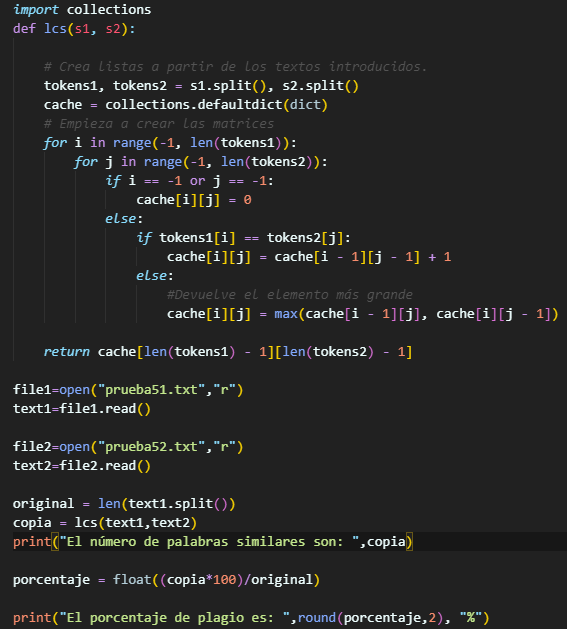
\includegraphics[width=1\textwidth]{codigo.png}
    \caption{Implementaci\'on del c\'odigo}
    \label{fig:codigo}
\end{figure}

\begin{figure}
    \centering
    \textit{Lorem ipsum dolor sit amet, consectetur adipiscing elit. 
Curabitur mollis, neque quis dignissim fringilla, arcu sem 
efficitur elit, nec finibus dui felis sed augue. In et consectetur 
felis, venenatis mattis ligula. Etiam maximus bibendum viverra. 
Nullam nibh leo, tempus non consectetur eu, facilisis a turpis. 
Nam eget gravida felis, eu finibus ante. Aliquam a dictum elit. 
Aenean quam diam, finibus maximus dolor in, auctor feugiat dolor. 
Quisque et mollis nisl. Nam maximus velit libero, a tempus nulla 
cursus sit amet. Nulla eget tellus iaculis, finibus ligula non, 
aliquam leo. Vivamus blandit pretium posuere. Vestibulum fringilla 
accumsan nunc, sit amet malesuada risus efficitur id. Nulla 
lobortis eget tortor ac dignissim. Pellentesque purus dolor, 
pulvinar quis nulla sed, pellentesque molestie tellus. Sed rhoncus 
ac nibh eget tincidunt.}
    \caption{Texto original de la primera prueba}
    \label{fig:texto11}
\end{figure}

\begin{figure}
    \centering
    \textit{Lorem ipsum dolor sit amet, consectetur adipiscing elit. 
Curabitur mollis, neque quis dignissim fringilla, arcu sem 
efficitur elit, nec finibus dui felis sed augue. In et consectetur 
felis, venenatis mattis ligula. Etiam maximus bibendum viverra. 
Nullam nibh leo, tempus non consectetur eu, facilisis a turpis. 
Nam eget gravida felis, eu finibus ante. Aliquam a dictum elit. 
Aenean quam diam, finibus maximus dolor in, auctor feugiat dolor. 
Quisque et mollis nisl. Nam maximus velit libero, a tempus nulla 
cursus sit amet. Nulla eget tellus iaculis, finibus ligula non, 
aliquam leo. Vivamus blandit pretium posuere. Vestibulum fringilla 
accumsan nunc, sit amet malesuada risus efficitur id. Nulla 
lobortis eget tortor ac dignissim. Pellentesque purus dolor, 
pulvinar quis nulla sed, pellentesque molestie tellus. Sed rhoncus 
ac nibh eget tincidunt.}
    \caption{Texto de prueba de la primera prueba}
    \label{fig:texto12}
\end{figure}

\begin{figure}[ht]
    \centering
    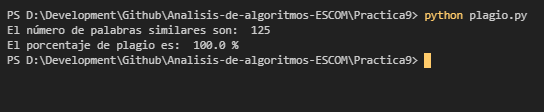
\includegraphics[width=1\textwidth]{1.png}
    \caption{Resultados de la primera prueba} 
    \label{fig:primera}
\end{figure}

\begin{figure}
    \centering
    \textit{Lorem ipsum dolor sit amet, consectetur adipiscing elit. 
Curabitur mollis, neque quis dignissim fringilla, arcu sem 
efficitur elit, nec finibus dui felis sed augue. In et consectetur 
felis, venenatis mattis ligula. Etiam maximus bibendum viverra. 
Nullam nibh leo, tempus non consectetur eu, facilisis a turpis. 
Nam eget gravida felis, eu finibus ante. Aliquam a dictum elit. 
Aenean quam diam, finibus maximus dolor in, auctor feugiat dolor. 
Quisque et mollis nisl. Nam maximus velit libero, a tempus nulla 
cursus sit amet. Nulla eget tellus iaculis, finibus ligula non, 
aliquam leo. Vivamus blandit pretium posuere. Vestibulum fringilla 
accumsan nunc, sit amet malesuada risus efficitur id. Nulla 
lobortis eget tortor ac dignissim. Pellentesque purus dolor, 
pulvinar quis nulla sed, pellentesque molestie tellus. 
Sed rhoncus ac nibh eget tincidunt.}
\textit{
Praesent eleifend pretium efficitur. Proin porttitor hendrerit 
turpis eu efficitur. In at luctus leo. Sed sed felis ut lacus 
facilisis pulvinar. Aliquam urna tellus, molestie eu urna eget, 
pharetra tempor ante. Praesent blandit, enim ac laoreet sollicitudin, 
magna lacus dictum orci, molestie vehicula nisl tortor commodo nisl. 
Aliquam erat volutpat. Vivamus fermentum eget lectus ac iaculis. 
Donec aliquet interdum odio sit amet rhoncus. Nam sed tortor orci. 
Fusce pellentesque eget felis eget lacinia. Phasellus metus risus, 
accumsan lobortis pulvinar nec, dictum vitae velit. Duis at dapibus 
tellus, a commodo dui. Nunc mi quam, sagittis a ultricies et, 
consectetur non ligula. Proin in tincidunt dolor, sed malesuada 
ipsum. Vestibulum ante ipsum primis in faucibus orci luctus et 
ultrices posuere cubilia Curae}
    \caption{Texto original de la segunda prueba}
    \label{fig:texto21}
\end{figure}

\begin{figure}
    \centering
    \textit{Nam maximus velit libero, a tempus nulla 
cursus sit amet. Nulla eget tellus iaculis, finibus ligula non, 
aliquam leo. Vivamus blandit pretium posuere. Vestibulum fringilla 
accumsan nunc, sit amet malesuada risus efficitur id. Nulla 
lobortis eget tortor ac dignissim. Pellentesque purus dolor, 
pulvinar quis nulla sed, pellentesque molestie tellus. 
Sed rhoncus ac nibh eget tincidunt.}
\textit{Praesent eleifend pretium efficitur. Proin porttitor hendrerit 
turpis eu efficitur. In at luctus leo. Sed sed felis ut lacus 
facilisis pulvinar. Aliquam urna tellus, molestie eu urna eget, 
pharetra tempor ante. Praesent blandit, enim ac laoreet sollicitudin, 
magna lacus dictum orci, molestie vehicula nisl tortor commodo nisl. 
Aliquam erat volutpat. Vivamus fermentum eget lectus ac iaculis. 
Donec aliquet interdum odio sit amet rhoncus. Nam sed tortor orci. 
Fusce pellentesque eget felis eget lacinia.}
    \caption{Texto de prueba de la segunda prueba}
    \label{fig:texto22}
\end{figure}

\begin{figure}[ht]
    \centering
    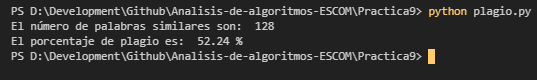
\includegraphics[width=1\textwidth]{2.png}
    \caption{Resultados de la segunda prueba} 
    \label{fig:segunda}
\end{figure}


\begin{figure}
    \centering
    \textit{In at luctus leo. Sed sed felis ut lacus 
facilisis pulvinar. Praesent blandit, enim ac laoreet sollicitudin, 
magna lacus dictum orci, molestie vehicula nisl tortor commodo nisl. 
Aliquam erat volutpat.}
\textit{Vestibulum fringilla 
accumsan nunc, sit amet malesuada risus efficitur id. Nulla 
lobortis eget tortor ac dignissim. Pellentesque purus dolor, 
pulvinar quis nulla sed, pellentesque molestie tellus. Sed rhoncus 
ac nibh eget tincidunt.}
    \caption{Texto original de la tercera prueba}
    \label{fig:texto31}
\end{figure}

\begin{figure}
    \centering
    \textit{Ut lacinia purus nec eros ultricies, a vulputate eros viverra. 
Curabitur ac ex quis tellus interdum sagittis. In blandit odio 
eget iaculis sagittis. Nullam sodales fermentum felis eu dapibus. 
Nulla elementum lacinia tempor. Maecenas mollis tincidunt sapien. 
Nam imperdiet est metus, quis egestas magna tempor id.}

\textit{Lorem ipsum dolor sit amet, consectetur adipiscing elit. 
Curabitur mollis, neque quis dignissim fringilla, arcu sem 
efficitur elit, nec finibus dui felis sed augue. In et consectetur 
felis, venenatis mattis ligula. Nam maximus velit libero, a tempus nulla 
cursus sit amet. Nulla eget tellus iaculis, finibus ligula non, 
aliquam leo. Vivamus blandit pretium posuere. Vestibulum fringilla 
accumsan nunc, sit amet malesuada risus efficitur id. Nulla 
lobortis eget tortor ac dignissim. Pellentesque purus dolor, 
pulvinar quis nulla sed, pellentesque molestie tellus. Sed rhoncus 
ac nibh eget tincidunt.}

\textit{Praesent eleifend pretium efficitur. Proin porttitor hendrerit 
turpis eu efficitur. In at luctus leo. Sed sed felis ut lacus 
facilisis pulvinar. Praesent blandit, enim ac laoreet sollicitudin, 
magna lacus dictum orci, molestie vehicula nisl tortor commodo nisl. 
Aliquam erat volutpat. Vivamus fermentum eget lectus ac iaculis. 
Donec aliquet interdum odio sit amet rhoncus.}

\textit{Aenean a nisi justo. Suspendisse sit amet dui commodo, 
suscipit nunc elementum, hendrerit erat. Etiam libero lectus, 
aliquam non ligula ut, condimentum semper tortor. Aliquam dapibus 
diam est, quis iaculis purus finibus sed. Aliquam erat volutpat. 
Aliquam eu libero auctor justo volutpat fermentum imperdiet sed 
velit. Nullam ultricies ante vitae lorem ultrices tincidunt. 
Quisque dignissim, lacus at faucibus laoreet, lacus tellus viverra 
leo, in gravida velit enim sed purus. Donec pharetra nisi augue, 
eget pretium turpis condimentum molestie.}
    \caption{Texto de prueba de la tercera prueba}
    \label{fig:texto32}
\end{figure}

\begin{figure}[ht]
    \centering
    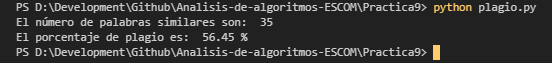
\includegraphics[width=1\textwidth]{3.png}
    \caption{Resultados de la tercera prueba} 
    \label{fig:tercera}
\end{figure}


\begin{figure}
    \centering
    \textit{Ut lacinia purus nec eros ultricies, a vulputate eros viverra. 
Curabitur ac ex quis tellus interdum sagittis. In blandit odio 
eget iaculis sagittis. Nullam sodales fermentum felis eu dapibus. 
Nulla elementum lacinia tempor. Maecenas mollis tincidunt sapien. 
Nam imperdiet est metus, quis egestas magna tempor id.}

\textit{Lorem ipsum dolor sit amet, consectetur adipiscing elit. 
Curabitur mollis, neque quis dignissim fringilla, arcu sem 
efficitur elit, nec finibus dui felis sed augue. In et consectetur 
felis, venenatis mattis ligula. Nam maximus velit libero, a tempus nulla 
cursus sit amet. Nulla eget tellus iaculis, finibus ligula non, 
aliquam leo. Vivamus blandit pretium posuere. Vestibulum fringilla 
accumsan nunc, sit amet malesuada risus efficitur id. Nulla 
lobortis eget tortor ac dignissim. Pellentesque purus dolor, 
pulvinar quis nulla sed, pellentesque molestie tellus. Sed rhoncus 
ac nibh eget tincidunt.}

\textit{Praesent eleifend pretium efficitur. Proin porttitor hendrerit 
turpis eu efficitur. In at luctus leo. Sed sed felis ut lacus 
facilisis pulvinar. Praesent blandit, enim ac laoreet sollicitudin, 
magna lacus dictum orci, molestie vehicula nisl tortor commodo nisl. 
Aliquam erat volutpat. Vivamus fermentum eget lectus ac iaculis. 
Donec aliquet interdum odio sit amet rhoncus.}


\textit{Aenean a nisi justo. Suspendisse sit amet dui commodo, 
suscipit nunc elementum, hendrerit erat. Etiam libero lectus, 
aliquam non ligula ut, condimentum semper tortor. Aliquam dapibus 
diam est, quis iaculis purus finibus sed. Aliquam erat volutpat. 
Aliquam eu libero auctor justo volutpat fermentum imperdiet sed 
velit. Nullam ultricies ante vitae lorem ultrices tincidunt. 
Quisque dignissim, lacus at faucibus laoreet, lacus tellus viverra 
leo, in gravida velit enim sed purus. Donec pharetra nisi augue, 
eget pretium turpis condimentum molestie.}
    \caption{Texto original de la cuarta prueba}
    \label{fig:texto41}
\end{figure}

\begin{figure}
    \centering
    \textit{Praesent eleifend pretium efficitur. Proin porttitor hendrerit 
turpis eu efficitur. In at luctus leo. Sed sed felis ut lacus 
facilisis pulvinar. Vivamus fermentum eget lectus ac iaculis. 
Donec aliquet interdum odio sit amet rhoncus.}
    \caption{Texto de prueba de la cuarta prueba}
    \label{fig:texto42}
\end{figure}

\begin{figure}[ht]
    \centering
    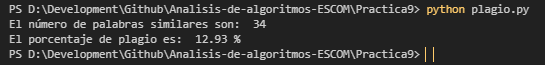
\includegraphics[width=1\textwidth]{4.png}
    \caption{Resultados de la cuarta prueba} 
    \label{fig:cuarta}
\end{figure}


Como hemos podido observar en esta cuarta prueba, en la figura  \ref{fig:texto42} se ha cambiado el orden de una oraci\'on respecto al texto mostrado en la figura \ref{fig:texto41}, lo que nos lleva al resultado mostrado en la figura \ref{fig:cuarta} donde no detecta similitud alguna, puesto que la implementaci\'on dada en esta pr\'actica aun no reconoce patrones y su an\'alisis de los textos los hace de forma "\textit{lineal}".

\begin{figure}
    \centering
    \textit{Ut lacinia purus nec eros ultricies, a vulputate eros viverra. 
Curabitur ac ex quis tellus interdum sagittis. In blandit odio 
eget iaculis sagittis. Nullam sodales fermentum felis eu dapibus. 
Nulla elementum lacinia tempor. Maecenas mollis tincidunt sapien. 
Nam imperdiet est metus, quis egestas magna tempor id.}

\textit{Aenean a nisi justo. Suspendisse sit amet dui commodo, 
suscipit nunc elementum, hendrerit erat. Etiam libero lectus, 
aliquam non ligula ut, condimentum semper tortor. Aliquam dapibus 
diam est, quis iaculis purus finibus sed. Aliquam erat volutpat. 
Aliquam eu libero auctor justo volutpat fermentum imperdiet sed 
velit. Nullam ultricies ante vitae lorem ultrices tincidunt. 
Quisque dignissim, lacus at faucibus laoreet, lacus tellus viverra 
leo, in gravida velit enim sed purus. Donec pharetra nisi augue, 
eget pretium turpis condimentum molestie.}
    \caption{Texto original de la quinta prueba}
    \label{fig:texto51}
\end{figure}

\begin{figure}
    \centering
    \textit{Lorem ipsum dolor sit amet, consectetur adipiscing elit. 
Curabitur mollis, neque quis dignissim fringilla, arcu sem 
efficitur elit, nec finibus dui felis sed augue. In et consectetur 
felis, venenatis mattis ligula. Nam maximus velit libero, a tempus nulla 
cursus sit amet. Nulla eget tellus iaculis, finibus ligula non, 
aliquam leo. Vivamus blandit pretium posuere. Vestibulum fringilla 
accumsan nunc, sit amet malesuada risus efficitur id. Nulla 
lobortis eget tortor ac dignissim. Pellentesque purus dolor, 
pulvinar quis nulla sed, pellentesque molestie tellus. Sed rhoncus 
ac nibh eget tincidunt.}

\textit{Praesent eleifend pretium efficitur. Proin porttitor hendrerit 
turpis eu efficitur. In at luctus leo. Sed sed felis ut lacus 
facilisis pulvinar. Praesent blandit, enim ac laoreet sollicitudin, 
magna lacus dictum orci, molestie vehicula nisl tortor commodo nisl. 
Aliquam erat volutpat. Vivamus fermentum eget lectus ac iaculis. 
Donec aliquet interdum odio sit amet rhoncus.}
    \caption{Texto de prueba de la quinta prueba}
    \label{fig:texto52}
\end{figure}

\begin{figure}[ht]
    \centering
    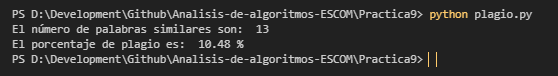
\includegraphics[width=1\textwidth]{5.png}
    \caption{Resultados de la quinta prueba} 
    \label{fig:quinta}
\end{figure}

\newpage
\section{Conclusiones}
\textit{Alan Romero Lucero}. Con esta pr\'actica se puede ver claramente el poder de la programaci\'on din\'amica en la resoluci\'on de problemas que implican el mundo real. Tambi\'en, creo que la soluci\'on planteada no es la \'optima, debido al consumo de recusros; tel vez para unas frases no habr\'a problema, pero para documentos grandes y extensos creo que representar\'a una cuesti\'on a considerar.
\newline\newline

\textit{Josu\'e David Hern\'andez Ram\'irez}. Como hemos podido analizar y observar dentro de esta pr\'actica, la implementaci\'on de la programaci\'on din\'amica ayuda a que el consumo de recursos sea mas eficiente a contrario del uso de la fuerza bruta para el an\'alisis o encontrar patrones como lo hemos implementado en esta pr\'actica.
\newline\newline
Creo que esto es la base de las herramientas profesionales que usan para detectar los plagios en los trabajos de los estudiantes y si se llega a implementar las redes neuronales o el machine learning para encontrar patrones para que la detecci\'on del plagio, la eficacia para su objetivo planteado en esta pr\'actica aumentar\'a bastante y har\'a que gane fiabilidad.


\section{Bibliograf\'ia}

[1]"Dynamic Programming in NLP - Longest Common Subsequence", Stokastik, 2018. [Online]. Available: http://www.stokastik.in/dynamic-programming-in-natural-language-processing-longest-common-subsequence/. [Accessed: 13- Nov- 2019].


\end{document}